\documentclass[
    oneside,            % Bez pustych stron wstawek (twoside + \cleardoublepage)
    left=2.5cm,         % Sadly, generic margin parameter
    right=2.5cm,        % doesnt't work, as it is
    top=2.5cm,          % superseded by more specific
    bottom=3cm,         % left...bottom parameters.
    bindingoffset=6mm,  % Optional binding offset.
    nohyphenation=false % You may turn off hyphenation, if don't like.
]{eiti/eiti-report}
\usepackage{tabularx}
\usepackage{ragged2e}
\langpol % Dla języka angielskiego mamy \langeng
\graphicspath{{img/}}             % Katalog z obrazkami.
\addbibresource{bibliografia.bib} % Plik .bib z bibliografią
\usepackage{setspace}
\setlength{\emergencystretch}{2em}

\begin{document}
\przedmiot{ORKUZ}
\reportDescription{Raport z projektu symulacyjnego iFogSim}
\title{
    Projekt 27 ORKUZ --- iFogSim
}

\author{Szymon Bedeniczuk, Adrian Chmiel, Michał Bogucki}
\date{\today}
\maketitle

\newpage

\tableofcontents

\clearpage
\pagestyle{headings}

\section{Wprowadzenie}
Fog Computing, pojęcie wprowadzone przez Cisco, oraz Edge Computing są modelami obliczeń rozproszonych rozszerzającymi koncepcję Cloud Computingu. Umożliwiają one przeniesienie części przetwarzania danych z centralnej chmury bliżej urządzeń brzegowych, takich jak routery, bramy IoT czy lokalne serwery, oraz bliżej źródeł danych i użytkowników końcowych. Komponenty aplikacji mogą działać w sposób rozproszony, korzystając z usług świadczonych przez infrastrukturę rozproszoną, w której zasady zarządzania zasobami kontrolują i zarządzają usługami oferowanymi przez każde urządzenie. 
Rozwiązanie to zapewnia większą gęstość zasobów, co pozwala ograniczyć opóźnienia w aplikacjach mobilnych, które często wymagają krótkiego czasu reakcji. Zwiększa ono również skalowalność systemu, ponieważ zmniejsza obciążenie centralnych serwerów chmurowych, umożliwia rozwój infrastruktury o kolejne urządzenia brzegowe oraz ogranicza ilość danych przesyłanych do chmury. Wykorzystanie fog computingu pomaga także w działaniu aplikacji krytycznych, wymagających przetwarzania danych w czasie rzeczywistym.

\section{Cel i Zastosowanie}
iFogSim to narzędzie stworzone do modelowania i symulacji środowisk Fog, Edge computing oraz Internet of Things (IoT), zbudowane na fundamentach frameworku CloudSim, narzędzia do symulowania środowisk Cloud. Narzędzie docelowo umożliwia testowanie i ocenę strategii zarządzania symulowanymi zasobami przed stworzeniem rzeczywistej infrastruktury.

Głównym celem iFogSim jest prowadzenie symulacji związanych z rozmieszaniem modułów aplikacji w środowiskach Fog i Edge w celu optymalizacji prędkości przesyłania danych między urządzeniami, harmonogramem ich zadań, analizą latencji, zużyciem energii, oraz wykorzystaniem sieci w infrastrukturze~\cite{iFogSimTut}.

Narzędzie iFogSim wykorzystywane już było w symulacjach infrastruktur np. inteligentnych budynków, w których wiele systemów musi współpracować ze sobą, oraz działać przy jak najmniejszej latencji~\cite{iFogSimSmartBuilding}.

Kolejnym przykładem wykorzystania tego narzędzia jest infrastruktura medyczna mająca na celu monitorowanie pacjentów w czasie rzeczywistym. To zastosowanie jest przykładem sytuacji, w której niska latencja jest najważniejsza, gdyż może od niej zależeć zdrowie lub życie pacjenta~\cite{HealthCare}.

Ostatnim przykładem będzie monitoring wideo w smart city. W takim zastosowaniu kluczowe znaczenie ma rejestrowanie obrazu i dźwięku, a następnie ich analiza w celu wykrywania zagrożeń. Wymaga to szybkiego przetwarzania danych w czasie rzeczywistym. Badacze porównali rozwiązania bazujące na modelach Cloud Computing i Fog Computing, przy czym Fog okazał się bardziej korzystny~\cite{SmartCity}.

Przedstawione przykłady pokazują, że iFogSim jest wykorzystywany przede wszystkim do testowania rozwiązań typu fog w dwóch przypadkach. Pierwszy dotyczy systemów, które obecnie opierają się na infrastrukturze chmurowej. Drugi obejmuje rozwiązania integrujące wiele powiązanych ze sobą zastosowań, w których kluczowe znaczenie mają optymalizacja oraz koordynacja ich działania.

\section{Architektura Narzędzia}
iFogSim składa się z warstw, które współpracują ze sobą, odpowiadając za określone zadania oraz zapewniając prawidłowe działanie systemu. Odzwierciedlają one architekturę IoT, w której urządzenia generują dane, a następnie przekazują je do wyższych warstw. Po przeprowadzeniu analizy system może przesłać odpowiednie zadania do urządzeń wykonawczych.~\cite{iFogSimInf}. 

\begin{figure}[htbp]
    \centering
    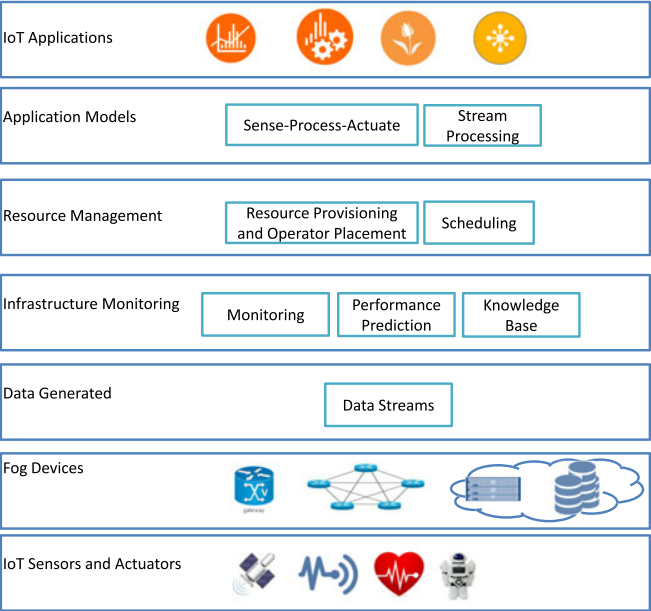
\includegraphics[width=\linewidth,keepaspectratio]{architekturaiFogSim.png}
    \caption{Architektura narzędzia iFogSim, wykorzystane ze strony \url{https://onlinelibrary.wiley.com/}.}
\end{figure}
Poniższe podrozdziały opisują kolejno warstwy widoczne na rysunku — od urządzeń IoT u dołu, przez Fog i strumień danych, aż po monitorowanie, zarządzanie zasobami i aplikacje u góry hierarchii.

\subsection{Warstwa urządzeń IoT}
Urządzenia IoT stanowią najniższą warstwę architektury, gdyż są zestawem urządzeń odpowiedzialnych za kontakt z użytkownikiem. Przykładami urządzeń z tej warstwy są między innymi urządzenia zbierające dane, takie jak sensory, kamery, mikrofony itd. Aktuatory również należą do tej kategorii. Odpowiadają za wykonywanie określonych działań, takich jak sterowanie oświetleniem, głośnikami, zamkami lub alarmami. Ich praca jest sterowana przez urządzenia znajdujące się w wyższych warstwach architektury.

\subsection{Warstwa urządzeń Fog}
Kolejną warstwą w środowisku są urządzenia fog, które zajmują się przetwarzaniem otrzymanych danych oraz wysyłaniem sygnałów do urządzeń warstwy niższej. Do tych urządzeń należą bramy sieciowe, routery, oraz lokalne serwery. Urządzenia z tej warstwy również podlegają wewnętrznej hierarchii. Urządzenia najbliższe użytkownikowi to routery i bramy sieciowe. Wyżej w hierarchii są lokalne serwery, urządzenia pomiędzy użytkownikiem a chmurą. Na najwyższym poziomie tej architektury znajduje się chmura obliczeniowa.
Z tym stanem wiąże się też fakt, że urządzenia na tym samym poziomie hierarchii nie komunikują się ze sobą. Ciąg komunikacyjny idzie z góry do dołu, w parze parent-child. Struktura ta może przypominać drzewo.

\subsection{Warstwa wygenerowanych danych}
Warstwa danych jest szeroko pojętym strumieniem danych przesyłanym pomiędzy poprzednimi dwoma warstwami a szerszym systemem oraz z powrotem, a także pomiędzy urządzeniami wyższych warstw, które odpowiadają za warstwę aplikacyjną. Takimi danymi mogą być odczyty z sensorów, dane z aplikacji urządzeń fog, informacje przesyłane do urządzeń IoT, aktualizacje ich działania oraz inne komunikaty systemowe.

\subsection{Warstwa monitorowania infrastruktury}
Warstwa ta odpowiada za zbieranie i monitorowanie danych dotyczących obciążenia infrastruktury. Do tych danych zalicza się wykorzystanie zasobów podzespołów, przepustowość sieci, zużycie energii, oraz informacje o stanie urządzeń IoT, oraz ich aktywności. Dane te, po zebraniu przekazywane są do warstwy zarządzania zasobami, albo być przekazane innym servisom w ramach potrzeby.
\subsection{Warstwa zarządzania zasobami}
Zarządzanie zasobami jest głównym komponentem infrastruktury. Obejmuje ono mechanizmy odpowiedzialne za zarządzanie zasobami warstwy urządzeń fog, tak aby spełnić wymagania warstwy aplikacyjnej przy możliwie najmniejszym wykorzystaniu zasobów. 
Warstwa korzystając z informacji na temat zasobów zebrane z warstwy poprzedniej identyfikuje najlepsze możliwe urządzenia do hostowania aplikacji, oraz alokowania zasobów na nich. Warstwa ta może również definiować reguły zarządzania infrastrukturą, których celem jest możliwie efektywne wykorzystanie dostępnych zasobów. Mogą one być za równo skomplikowane, na przykład mające na celu wprowadzanie dynamicznych zmian w systemie w czasie rzeczywistym, lub proste, jak zwyczajnie, takie jak rozłożenie całej infrastruktury po równo w każdym urządzeniu.
Zarządzanie zasobami może być także dystrybuowane, w takiej sytuacji każde z urządzeń może się zarządzać samo, bez wiedzy reszty infrastruktury, lub centralizowane, gdzie wszystkim zarządza jeden system.

\subsection{Warstwa aplikacji}
Jest to warstwa samych aplikacji przeznaczonych do infrastruktury fog, a przez to do modelu rozproszonego przepływu danych (DDF)~\cite{DDF}. W modelu przepływu danych logikę aplikacji można przedstawić jako ukierunkowany graf, w którym każdy wierzchołek może reprezentować moduł wejściowy, moduł wyjściowy lub niezależny moduł przetwarzający. Pozwala to na dynamiczne dodawanie lub usuwanie wierzchołków oraz na ich funkcjonalność.
W iFogSim aplikację opisuje klasa Application, w której moduły AppModule mają przypisane wymagania dotyczące mocy obliczeniowej, pamięci RAM oraz przepustowości. Krawędzie grafu AppEdge łączą sensory, moduły i aktuatory, określając kierunek przepływu danych w górę lub w dół hierarchii oraz rozmiar przesyłanych krotek (tuples). Zamknięte ścieżki przetwarzania definiuje AppLoop, co pozwala mierzyć opóźnienie całego cyklu w eksperymentach przypisywania modułów do urządzeń.
Taki model dataflow stanowi punkt wyjścia dla wszystkich scenariuszy symulacyjnych opisanych dalej w raporcie.

\section{Przegląd literatury}
W literaturze dotyczącej iFogSim można wyróżnić trzy podstawowe publikacje, które stanowią punkt odniesienia dla dalszej części pracy.
Pierwsza z nich~\cite{iFogSimSPE} przedstawia oryginalny toolkit iFogSim jako rozszerzenie CloudSim do modelowania zarządzania zasobami w IoT, Edge i Fog. Autorzy opisują hierarchię urządzeń, model aplikacji DDF oraz sposób rozmieszczania modułów, co stanowi podstawę naszych eksperymentów porównujących strategie Cloud i Fog. Należy jednak pamiętać, że oryginalny artykuł nie uwzględniał mobilności urządzeń, wykorzystywał uproszczony model energii, a wyniki symulacji zależały od ręcznie dobranych parametrów MIPS.
Kolejna praca~\cite{iFogSim2JSS} rozszerza możliwości symulatora o obsługę urządzeń mobilnych, grupowanie mikroserwisów w klastry oraz mechanizmy migracji, co jest istotne zwłaszcza w scenariuszu CrowdSensing. Z analizy tej publikacji wynika, że samo rozszerzenie symulatora o mobilność nie oznacza jeszcze automatycznej przewagi Fog nad Cloud. Nasze wyniki CrowdSensing pokazują to wyraźnie: przy małej liczbie użytkowników dominuje narzut migracji, w średniej skali widać korzyść z lokalnego przetwarzania, a przy dużym obciążeniu przetwarzanie brzegowe nie zapewnia już tak wyraźnych korzyści. Wadą tego rozszerzenia jest przy tym rosnąca złożoność konfiguracji, gdyż koszt migracji modułów może zdominować korzyść Fog przy małej skali obciążenia.
Rozdział tutorialowy~\cite{iFogSimTutBook} w opracowaniu Buyya i Srirama porządkuje sposób budowania topologii, definiowania aplikacji oraz zbierania metryk, takich jak latencja, energia czy wykorzystanie sieci. W naszym projekcie zastosowaliśmy podobne podejście: jawne definiowanie pętli aplikacyjnych, zapis wyników do plików CSV oraz porównanie placementu Cloud-only z placementem Fog opartym na ModulePlacementEdgewards. Tutorial opisuje API symulatora, lecz nie dostarcza walidacji na danych produkcyjnych ani gotowych benchmarków dla wszystkich domen IoT, dlatego w projekcie sami zdefiniowaliśmy scenariusze eksperymentalne.
Podsumowując przegląd literatury, korzyść z Fog zależy od tego, jak dobrze dopasowane są zasoby brzegowe do obciążenia (DCNS), jak kosztowna jest migracja (CrowdSensing) oraz jak złożony jest przepływ danych w aplikacji (nasz scenariusz monitoringu środowiskowego). Przeniesienie obliczeń bliżej urządzeń IoT bez sprawdzenia nasycenia MIPS może dać wynik taki sam jak w chmurze albo nawet gorszy pod względem zużycia energii.

\section{Interfejs programowania}
W naszym forku iFogSim interfejs programowania służy do zbudowania topologii urządzeń, zdefiniowania aplikacji oraz uruchomienia symulacji z wybraną strategią rozmieszczania modułów. Poniżej opisano elementy API wykorzystane we wszystkich czterech scenariuszach eksperymentalnych.

\subsection{Struktura kodu}
Kod źródłowy iFogSim jest podzielony na pakiety odpowiadające poszczególnym warstwom symulatora. Tabela~\ref{tab:packages} zestawia najważniejsze z nich wraz z rolami i klasami używanymi w naszych eksperymentach.
iFogSim dziedziczy po CloudSim model zdarzeń dyskretnych — DES, w którym cała symulacja to sekwencja zdarzeń kolejkowanych przez silnik \texttt{CloudSim}. Encje symulacji – urządzenia Fog, sensory i aktuatory – rejestruje \texttt{FogBroker}, a przetwarzanie krotek oraz rozliczenie zużycia zasobów odbywają się asynchronicznie w pętli zdarzeń.

Harmonogramowanie modułów aplikacji na hoście obliczeniowym \texttt{PowerHost} realizuje \texttt{Stream\-Operator\-Scheduler}, który decyduje o kolejności obsługi operatorów strumieniowych. Dzięki temu można porównywać strategie rozmieszczenia modułów w tych samych warunkach topologicznych.

\begin{table}[htbp]
\centering
\scriptsize
\setlength{\tabcolsep}{3pt}
\renewcommand{\arraystretch}{1.1}
\begin{tabularx}{\textwidth}{|>{\raggedright\arraybackslash}p{0.26\textwidth}|>{\raggedright\arraybackslash}p{0.14\textwidth}|>{\raggedright\arraybackslash}X|}
\hline
Pakiet & Rola & Kluczowe klasy \\
\hline
\texttt{org.cloudbus.cloudsim} & Silnik DES & \texttt{CloudSim}, \texttt{SimEntity}, \texttt{PowerHost} \\
\texttt{org.fog.entities} & Topologia & \texttt{FogDevice}, \texttt{Sensor}, \texttt{Actuator}, \texttt{Tuple}, \texttt{FogBroker} \\
\texttt{org.fog.application} & Model DDF & \texttt{Application}, \texttt{AppModule}, \texttt{AppEdge}, \texttt{AppLoop} \\
\texttt{org.fog.placement} & Placement & \texttt{Controller}, \texttt{ModulePlacementMapping}, \texttt{ModulePlacementEdgewards} \\
\texttt{org.fog.utils} & Metryki & \texttt{TimeKeeper}, \texttt{NetworkUsageMonitor}, \texttt{Config} \\
\texttt{org.fog.scheduler} & Harmonogram & \texttt{StreamOperatorScheduler} \\
\texttt{org.fog.test.perfeval} & Eksperymenty & \texttt{DCNSFog}, \texttt{CrowdSensing\_*}, \texttt{EnvironmentalMonitoringFog}, \texttt{VRGameFog} \\
\hline
\end{tabularx}
\caption{Główne pakiety iFogSim wykorzystane w projekcie.}
\label{tab:packages}
\end{table}

\subsection{Klasy infrastruktury}
Węzły infrastruktury reprezentuje klasa FogDevice, która określa m.in. moc obliczeniową (MIPS), pamięć RAM, przepustowość i model zużycia energii. Sensory i aktuatory generują oraz odbierają krotki danych według zadanego rozkładu czasu, na przykład stałego interwału — DeterministicDistribution. Encje symulacji rejestruje FogBroker w ramach CloudSim.

\subsection{Warstwa aplikacji i sterowanie}
Aplikację tworzy się przez dodanie modułów, krawędzi przepływu danych oraz mapowań krotek między modułami. AppLoop wyznacza ścieżkę, dla której mierzone jest opóźnienie end-to-end. Symulację uruchamia Controller.submitApplication z wybranym placementem: ModulePlacementMapping umieszcza wszystkie moduły w chmurze, natomiast ModulePlacementEdgewards próbuje wykorzystać zasoby urządzeń Fog bliżej źródła danych.
W trakcie symulacji zbierane są m.in. opóźnienia pętli – TimeKeeper, wykorzystanie sieci – NetworkUsageMonitor oraz energia zużyta przez poszczególne urządzenia FogDevice.

\subsection{Interfejs wiersza poleceń i eksport wyników}
Aplikacje testowe z katalogu \texttt{perfeval} rozszerzyliśmy o argumenty wiersza poleceń, dzięki czemu ten sam plik \texttt{.java} można uruchamiać w wielu konfiguracjach bez ponownej kompilacji.

\begin{itemize}[noitemsep,topsep=2pt]
    \item \textbf{DCNS}: \texttt{--areas}, \texttt{--cameras}, \texttt{--cloud}
    \item \textbf{CrowdSensing}: \texttt{--users}, \texttt{--cloud-only}
    \item \textbf{Monitoring środowiskowy}: \texttt{--gateways}, \texttt{--sensors-per-gateway}, \texttt{--cloud}, opcjonalnie \texttt{--anomaly-selectivity}
    \item \textbf{VRGame}: \texttt{--departments}, \texttt{--mobiles-per-dept}, \texttt{--cloud}
\end{itemize}

Po zakończeniu symulacji wyniki dopisywane są do pliku CSV danego scenariusza. Zapis obejmuje opóźnienie pętli, wykorzystanie sieci, energię całkowitą i koszt wykonania w chmurze, a w DCNS dodatkowo osobno opóźnienie detekcji i śledzenia oraz opóźnienie sterowania PTZ — kolumny \texttt{Loop1Latency}, \texttt{Loop2Latency}.

\subsection{Skrypt eksperymentalny}
Uruchomienie wszystkich wariantów realizuje skrypt scripts/run\_experiments.sh. Kompiluje on zmodyfikowane klasy placementu oraz cztery aplikacje, a następnie uruchamia łącznie 224 warianty symulacji. Dla każdego wariantu obowiązuje limit czasu 10 minut, a pełne logi trafiają do katalogu logs/. Gotowe pliki CSV są przenoszone do katalogu results/.

\section{Aplikacje}
W projekcie wykorzystaliśmy cztery aplikacje symulacyjne. Trzy z nich pochodzą z oryginalnego repozytorium iFogSim — katalog perfeval, a czwartą — monitoring środowiskowy — zaimplementowaliśmy sami w ramach forka.

\subsection{DCNS – Intelligent Video Surveillance (oryginalna aplikacja)}
Klasa DCNSFog.java (autor: Harshit Gupta) modeluje monitoring wideo w smart city. Dane z kamer przechodzą przez detekcję ruchu, detektor obiektów i tracker; aplikacja ma dwie pętle pomiarowe: \emph{detekcji i śledzenia} (motion\_detector $\rightarrow$ object\_detector $\rightarrow$ object\_tracker) oraz \emph{sterowania PTZ} (object\_tracker $\rightarrow$ PTZ\_CONTROL). Topologia obejmuje chmurę, serwer proxy, routery obszarowe (2800 MIPS) oraz sensory kamer wysyłające dane co 5 ms.

\subsection{CrowdSensing --- mobilne mikroserwisy (oryginalna aplikacja)}
Klasa CrowdSensing\_Microservices\_RandomMobility\_Clustering.java symuluje mobilnych użytkowników korzystających z mikroserwisów i klastrowania. Aplikacja ma charakter upload-only, bez zamkniętej pętli do aktuatora, dlatego metryka AvgLoopLatency przyjmuje wartość $-1$\,ms. W analizie koncentrujemy się na ruchu sieciowym, energii oraz czasie migracji modułów.

\subsection[Monitoring środowiskowy]{EnvironmentalMonitoringFog --- monitoring środowiskowy (nasza aplikacja)}
Jako własny scenariusz zaimplementowaliśmy monitoring temperatury i wilgotności w budynku inteligentnym. Topologia jest statyczna, bez mobilności użytkowników i bez zewnętrznego zbioru danych. Przepływ danych przedstawiono na rysunku 6.1.
\begin{figure}[htbp]
    \centering
    \footnotesize
    \setlength{\fboxsep}{4pt}
    \resizebox{\linewidth}{!}{%
        \fbox{sensor środowiskowy} $\rightarrow$ \fbox{filtr danych}
        $\rightarrow$ \fbox{detektor anomalii}
        $\rightarrow$ \fbox{alarm}%
    }
    \caption{Graf przepływu danych aplikacji EnvironmentalMonitoringFog}
\end{figure}
Pętla pomiarowa obejmuje moduły od filtra do alarmu. Infrastruktura składa się z jednej chmury (44800 MIPS), jednego proxy (2800 MIPS, opóźnienie uplink 100 ms), wielu bram fog (2800 MIPS) oraz sensorów przypisanych do każdej bramy (interwał 10 ms). Przy \texttt{--cloud=true} wszystkie moduły trafiają do chmury; przy \texttt{--cloud=false} stosowany jest placement \texttt{Module\-Placement\-Edgewards} z początkowym mapowaniem filtra na bramy.

Dodatkową modyfikacją w forku jest parametr \texttt{--anomaly-selectivity}, który przez \texttt{FractionalSelectivity} na wyjściu modułu \texttt{anomaly\_detector} określa, jaki ułamek krotek docierających do detektora generuje alarm. W monitoringu środowiskowym większość odczytów jest normalna, więc ciężki detektor (1500 MIPS) nie powinien uruchamiać się dla każdej krotki. Domyślna wartość parametru wynosi 1,0, a w drugim przebiegu w fazie \texttt{env-sparse}, parametr został zredukowany do 0,1. W wynikowych danych energia Fog pozostaje taka sama, jak przy selektywności 1,0 (np. 12$\times$4: ok. 5\,407\,003\,W w obu fazach), natomiast ruch sieciowy Cloud maleje --- przy 12$\times$4 z ok. 263\,171 do ok. 238\,893 jednostek (ok. 9\%).

\subsection{VRGameFog --- VR/EEG (oryginalna aplikacja, rozszerzona)}
Kolejnym przykładem z katalogu perfeval jest klasa VRGameFog.java (autor: Harshit Gupta), modelująca grę VR sterowaną sygnałem EEG. Aplikacja ma jedną pętlę pomiarową: sensor EEG $\rightarrow$ klient $\rightarrow$ kalkulator stężenia $\rightarrow$ klient $\rightarrow$ aktuator, co odzwierciedla wymagania interaktywne — opóźnienie end-to-end decyduje o płynności sterowania. Moduł client emituje krotki typu \texttt{\_SENSOR} z selektywnością 0,9, gdyż nie każdy odczyt EEG wymaga pełnej analizy koncentracji.
Topologia obejmuje chmurę, serwer proxy, routery departamentowe oraz smartfony użytkowników. W strategii Cloud moduły, jak kalkulator stężenia i złącze trafiają do chmury, a klient pozostaje na urządzeniu mobilnym, za to w strategii Fog placement \texttt{ModulePlacementEdgewards} próbuje przesunąć obliczenia bliżej użytkownika. W forku dodaliśmy argumenty \texttt{--departments}, \texttt{--mobiles-per-dept} i \texttt{--cloud} oraz eksport wyników.

\section{Eksperymenty}
\subsection{Metodologia}
W każdym scenariuszu porównaliśmy dwie strategie rozmieszczania modułów. Pierwsza to prosty baseline Cloud-only, w którym moduły aplikacji wykonywane są w chmurze. Druga to placement Fog, w którym symulator próbuje wykorzystać urządzenia brzegowe zgodnie z dostępnymi zasobami MIPS.
Jako miary jakości przyjęliśmy opóźnienie pętli (w DCNS osobno: detekcja i śledzenie oraz sterowanie PTZ), wykorzystanie sieci, energię całkowitą oraz koszt wykonania w chmurze. Dla CrowdSensing dodatkowo mierzyliśmy czas migracji mikroserwisów.

\subsection{Zakres wariantów}
Dla CrowdSensing uruchomiono 28 różnych liczb użytkowników (od 1 do 100) w obu strategiach, co dało 56 wierszy w pliku CSV. Dla DCNS przetestowano 42 konfiguracje obszarów i kamer, również w wersjach Cloud i Fog, czyli 84 wiersze.

Własną aplikację uruchomiono w 14 konfiguracjach bram i sensorów w obu strategiach (28 wierszy przy selectivity 1,0, faza \texttt{env}) oraz ponownie w fazie \texttt{env-sparse} z \texttt{--anomaly-selectivity=0,1}, co dało łącznie 56 wierszy. Scenariusz VRGame obejmuje 14 konfiguracji departamentów i urządzeń mobilnych w wersji Cloud i Fog, czyli kolejne 28 wierszy danych.

Skrypt \texttt{run\_experiments.sh} wykonuje łącznie 224 symulacje: 84 DCNS + 56 CrowdSensing + 56 monitoring środowiskowy + 28 VRGame. Każda symulacja ma limit czasu, a szczegółowe logi zapisywane są w katalogu \texttt{logs}.

\subsection{Pułapki interpretacyjne}
Przy interpretacji wyników należy pamiętać o kilku efektach obserwowanych w danych. W DCNS, przy dużej liczbie kamer na obszar ($\geq$10), wartość około 3{,}02\,ms w kolumnie detekcji i śledzenia nie oznacza niskiego opóźnienia, lecz artefakt pomiaru przy nieukończonej pętli PTZ. W CrowdSensing wartość AvgLoopLatency równa $-1$ wynika z braku pętli zwrotnej i nie powinna być umieszczana na wykresach opóźnień. W VRGame przy dużej liczbie urządzeń mobilnych na departament, np. 5$\times$5, 8$\times$5, opóźnienia Fog i Cloud zbiegają się, co oznacza nasycenie routerów. Wreszcie, w niektórych konfiguracjach DCNS, np. 2$\times$25 i 3$\times$10, metryki Fog i Cloud są identyczne, co pokazuje, że sama obecność infrastruktury brzegowej nie wystarcza bez odpowiedniego wymiarowania zasobów.

\section{Wyniki}
\subsection[DCNS: Fog vs Cloud]{DCNS --- mapa korzyści Fog vs Cloud}
Poniższe wykresy przygotowano w notebooku \texttt{analysis/experiment\_analysis.ipynb} na podstawie plików CSV z katalogu \texttt{results/}.
\begin{figure}[htbp]
    \centering
    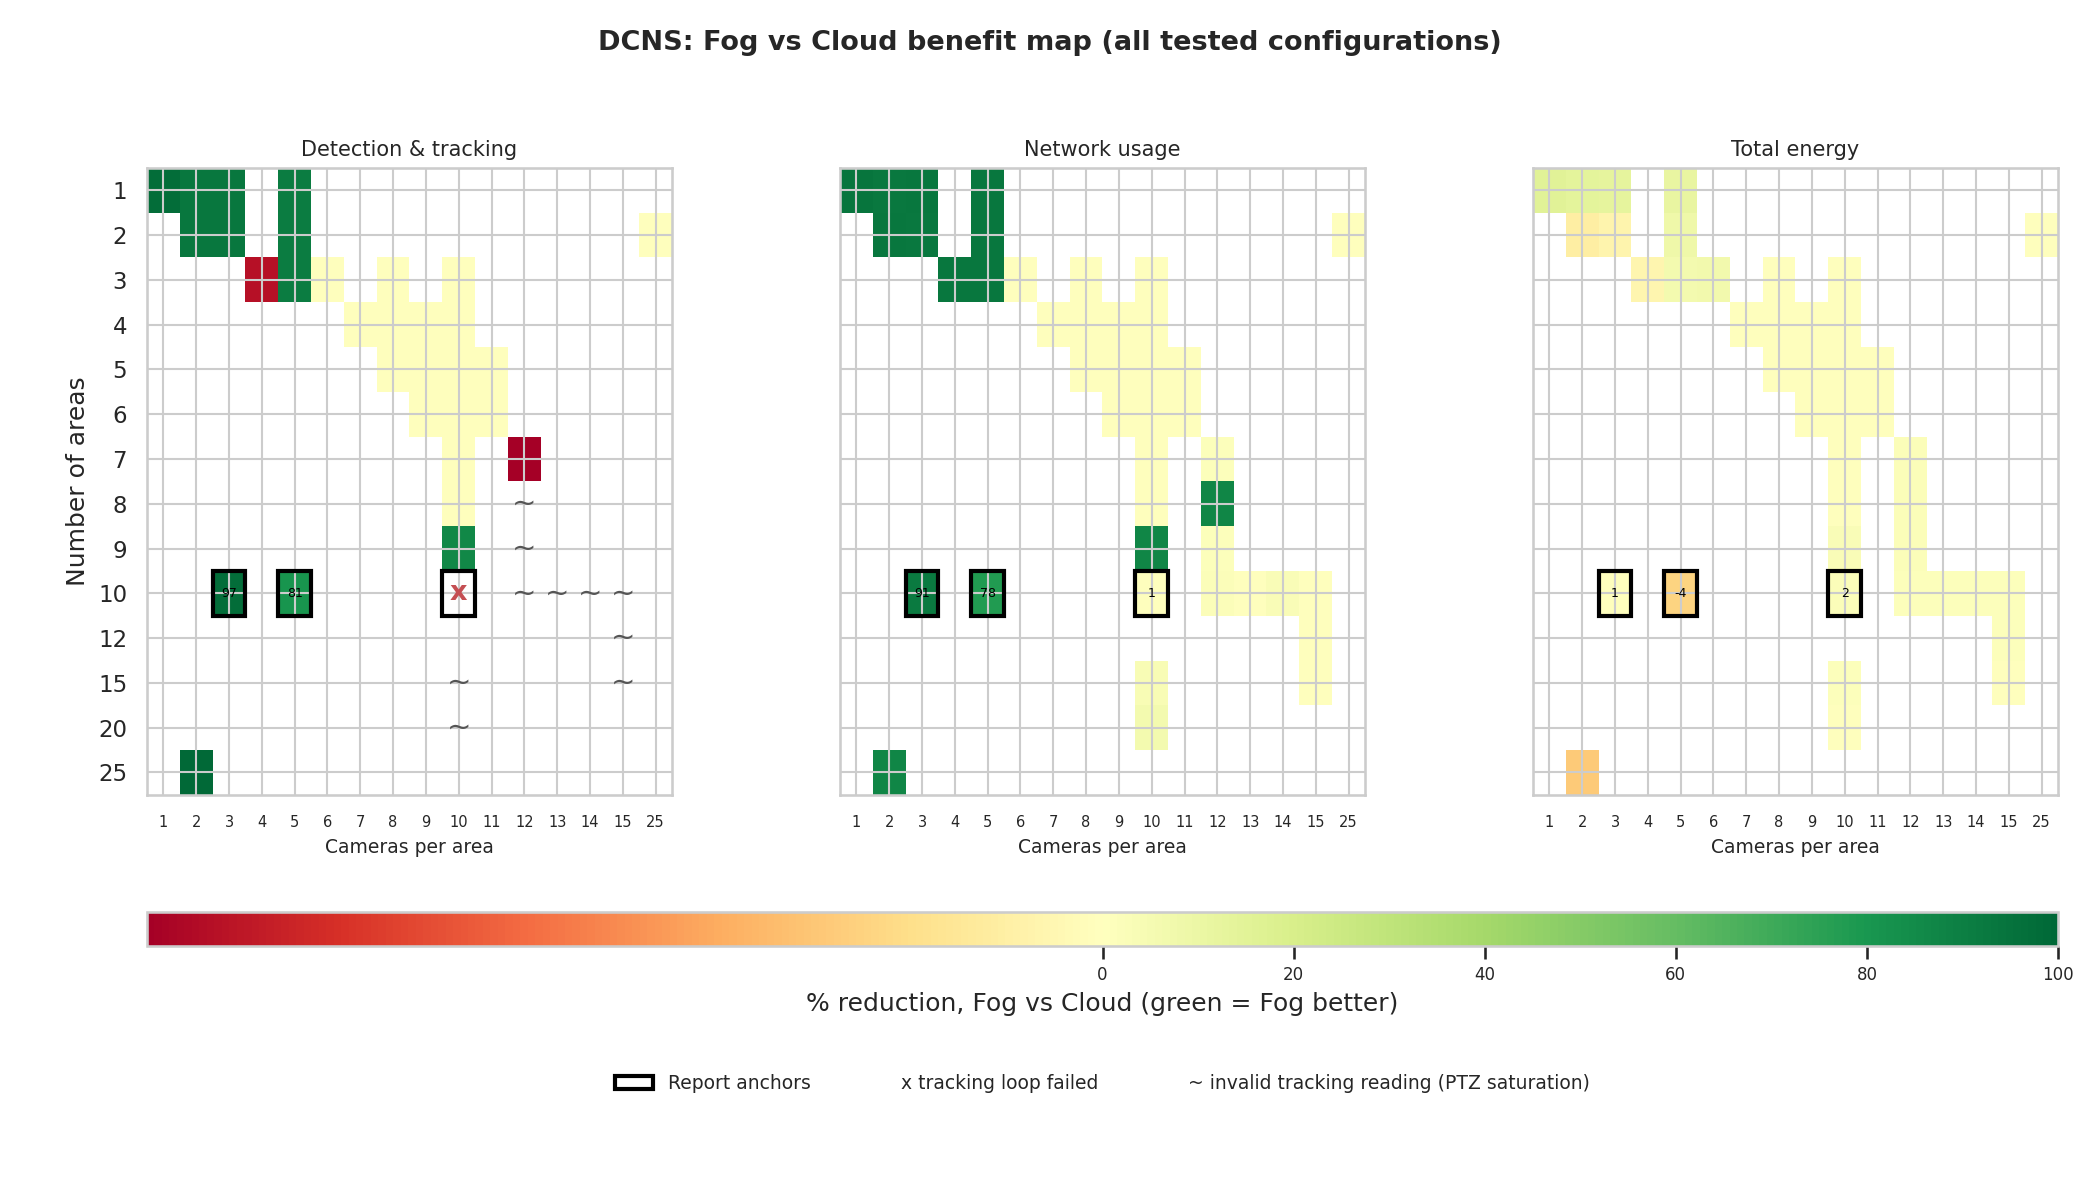
\includegraphics[width=\linewidth,keepaspectratio]{dcns_loop1_vs_cameras.png}
    \caption[Mapa korzyści DCNS]{Redukcja opóźnienia detekcji i śledzenia, ruchu sieciowego i energii (Fog względem Cloud) dla wszystkich testowanych konfiguracji. Ramki: punkty omawiane w tekście (10$\times$3, 10$\times$5, 10$\times$10); $\times$ --- brak ukończonej pętli detekcji; $\sim$ --- mylący odczyt (~3\,ms, nasycenie PTZ).}
\end{figure}

Przy małej liczbie kamer na obszar Fog daje wyraźną przewagę --- widać to jako zielone pola na mapie latencji i sieci. Dla konfiguracji 10$\times$3 opóźnienie detekcji i śledzenia spada z ok. 260{,}3\,ms w Cloud do ok. 7{,}2\,ms w Fog, co odpowiada redukcji około 97\%. Jednocześnie ruch sieciowy maleje o ok. 91\% (z ok. 1\,015\,587 do ok. 86\,637 jednostek).
Przy 5 kamerach na obszar (10$\times$5) Fog nadal skraca detekcję i śledzenie o ok. 81\%, ale energia rośnie o ok. 3{,}7\% względem Cloud, co pokazuje kompromis przy granicy zasobów routera.
\begin{figure}[htbp]
    \centering
    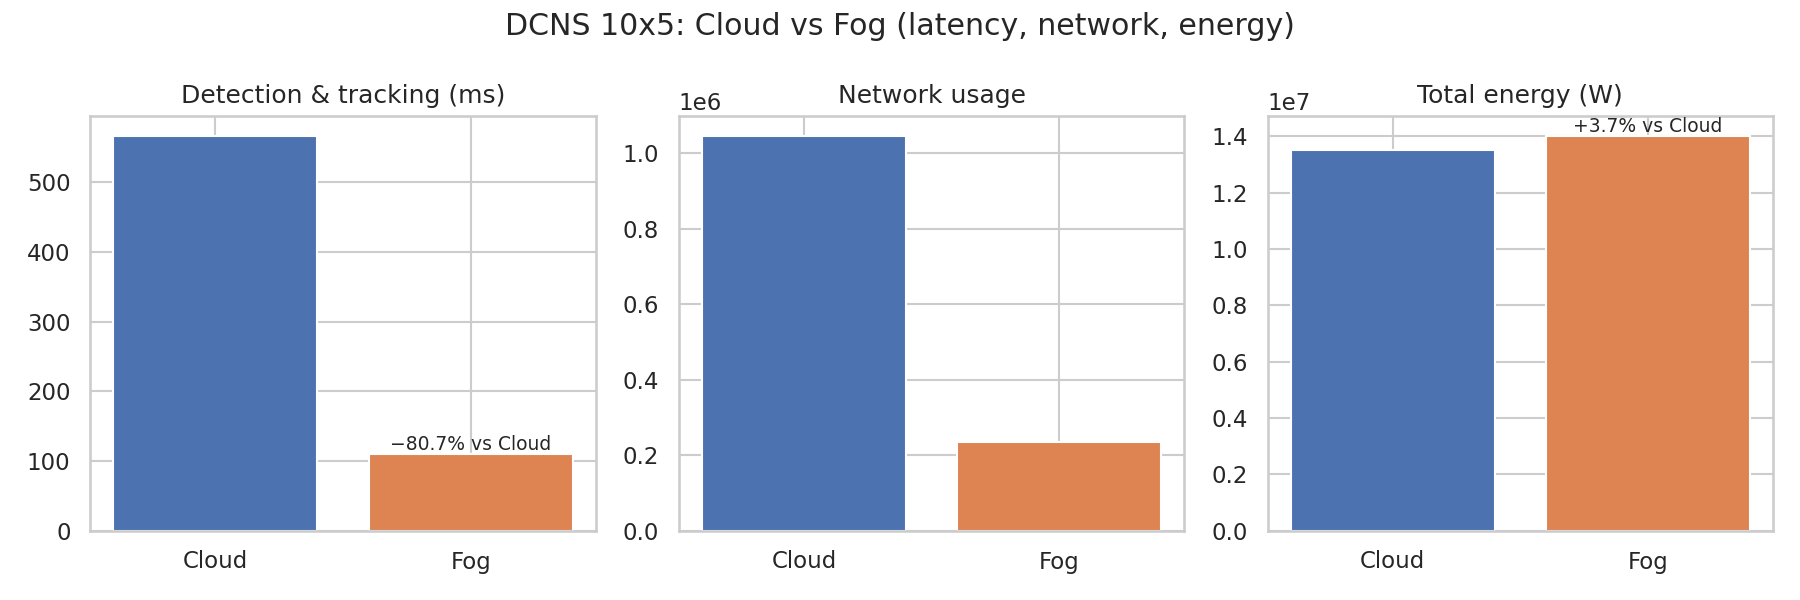
\includegraphics[width=\linewidth,keepaspectratio]{dcns_energy_anomaly.png}
    \caption{DCNS 10$\times$5: porównanie Cloud i Fog --- opóźnienie detekcji i śledzenia, ruch sieciowy i energia.}
\end{figure}
Jak widać na wykresie, przy konfiguracji 10$\times$5 Fog wyraźnie skraca opóźnienie detekcji i śledzenia i ogranicza ruch sieciowy względem Cloud, lecz jednocześnie zużywa nieco więcej energii (ok. +3{,}7\%). Ten kompromis ilustruje sytuację, gdy przesunięcie obliczeń na brzeg poprawia czas reakcji, ale obciąża lokalne routery przy granicy dostępnych MIPS. Konfiguracja 10$\times$10 jest punktem krytycznym: w strategii Fog nie ukończono żadnej z pętli --- detekcja i PTZ miały wartość $-1$.

\subsection[CrowdSensing: sieć i energia]{CrowdSensing --- ruch sieciowy i energia}
\begin{figure}[htbp]
    \centering
    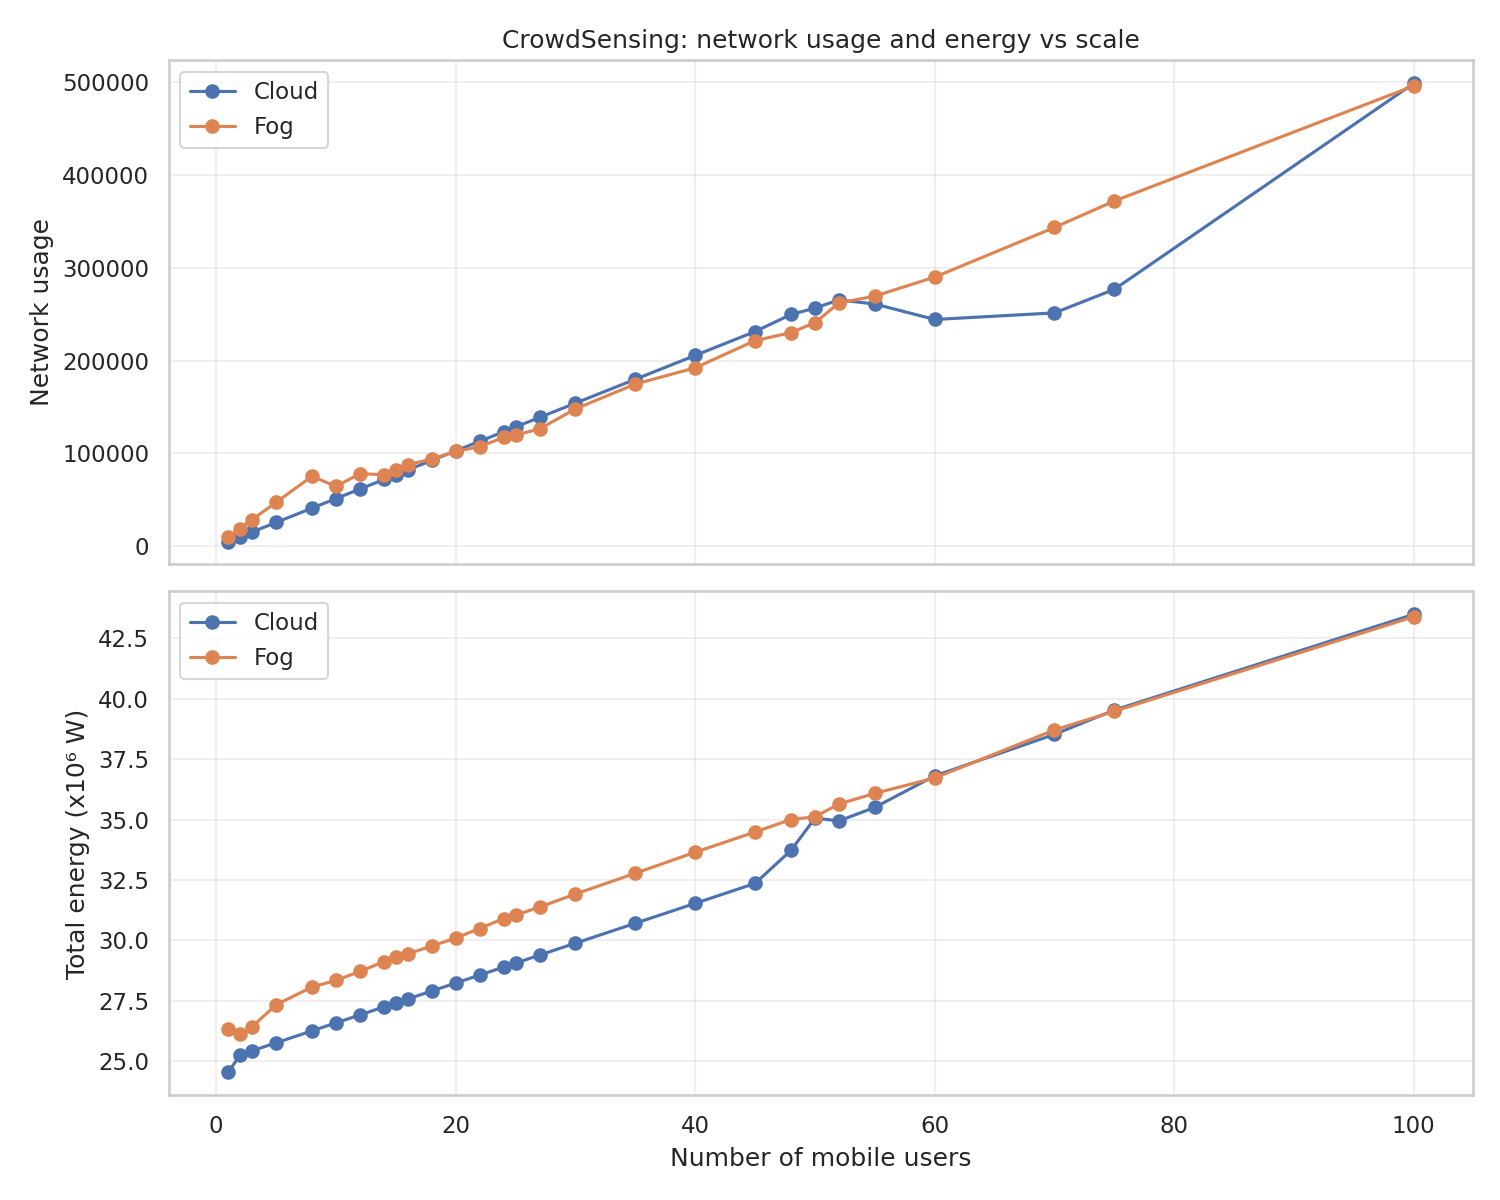
\includegraphics[width=\linewidth,keepaspectratio]{crowd_network_energy.png}
    \caption{Ruch sieciowy (góra) i całkowita energia (dół) w funkcji liczby użytkowników mobilnych dla strategii Cloud i Fog.}
\end{figure}

Jak widać na wykresie, przy małej liczbie użytkowników Fog generuje większy ruch sieciowy niż Cloud, m.in. z powodu migracji mikroserwisów, maksymalnie ok. +87\% przy 3 użytkownikach. Korzyść Fog pojawia się w okolicach 20 użytkowników, np. spadek ruchu o ok. 0{,}5\% względem Cloud przy przejściu z 18 do 20 użytkowników i utrzymuje się do ok. 50 użytkowników z maksymalną oszczędnością ok. 8{,}9\% przy 27 użytkownikach. Między 52 a 55 użytkownikami Fog znowu przegrywa sieciowo, np. +18{,}7\% przy 60 użytkownikach.
Na dolnym panelu widać, że energia Fog jest wyższa przy małej skali, np. +7{,}3\% przy 1 użytkowniku, lecz różnica maleje wraz ze wzrostem obciążenia; przy 100 użytkownikach Fog zużywa nieznacznie mniej energii od Cloud o ok. 0{,}2\%. Przy 70 użytkownikach czasy migracji wynoszą: Cloud 61{,}5\,ms, Fog 63{,}3\,ms.

\subsection[Monitoring: Fog vs Cloud]{Monitoring środowiskowy --- Fog vs Cloud}
\begin{figure}[htbp]
    \centering
    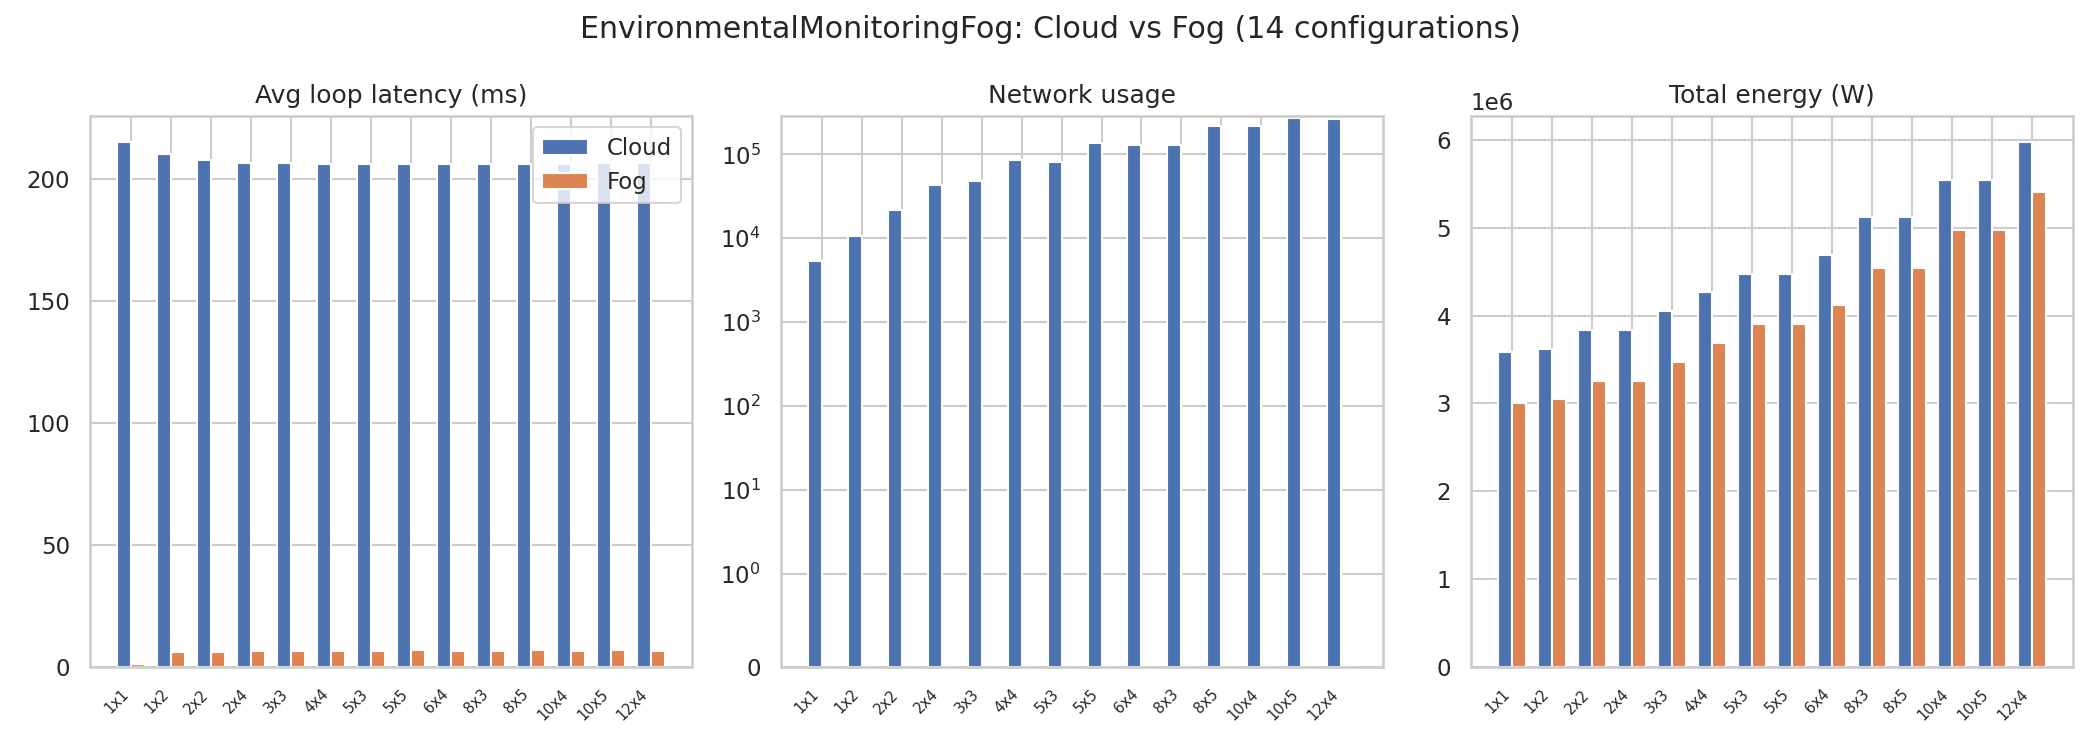
\includegraphics[width=\linewidth,keepaspectratio]{environmental_monitoring_fog_vs_cloud.png}
    \caption{Opóźnienie pętli, ruch sieciowy i energia dla 14 konfiguracji własnej aplikacji (faza \texttt{env}, selectivity 1,0).}
\end{figure}

We wszystkich przetestowanych konfiguracjach Fog osiąga niższe opóźnienie pętli niż Cloud. Dla najmniejszej skali 1$\times$1 latencja spada z ok. 215{,}1\,ms do ok. 1{,}2\,ms, co daje redukcję o ok. 99{,}4\%, a energia maleje o ok. 16{,}2\%. Przy większej konfiguracji 12$\times$4 redukcja opóźnienia wynosi ok. 96{,}8\%, a energia w Fog jest niższa o ok. 9{,}5\%.
W strategii Fog ruch sieciowy wynosi 0 we wszystkich wariantach, ponieważ przetwarzanie odbywa się lokalnie na bramach --- widać to na środkowym panelu wykresu. W Cloud dane muszą docierać do chmury, np. ok. 263\,171 jednostek ruchu przy 12$\times$4. W badanym zakresie nie zaobserwowano saturacji MIPS ani sytuacji, w której Fog dawałby wynik identyczny jak Cloud, co wiąże się z prostszym przepływem danych i mniejszymi wymaganiami obliczeniowymi modułów niż w scenariuszu DCNS.

Faza \texttt{env-sparse} (\texttt{--anomaly-selectivity=0,1}) powtórzyła te same 14 konfiguracji z rzadszym generowaniem sygnałów alarmowych.
\begin{figure}[htbp]
    \centering
    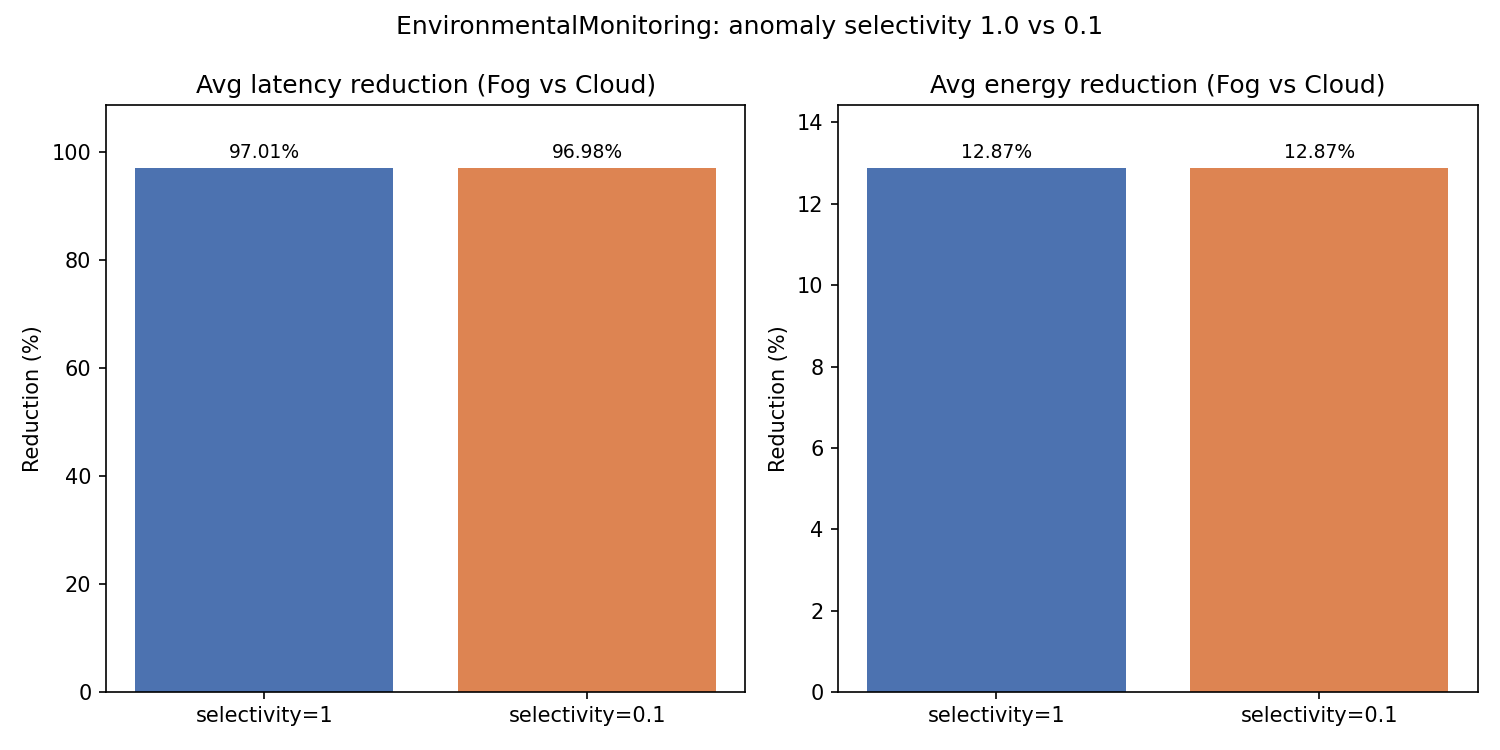
\includegraphics[width=\linewidth,keepaspectratio]{env_selectivity_comparison.png}
    \caption{Średnia redukcja opóźnienia i energii (Fog względem Cloud) dla selectivity 1,0 i 0,1, uśredniona po 14 konfiguracjach.}
\end{figure}
Jak widać na wykresie, korzyść Fog w opóźnieniu o ok. 97\% i energii o ok. 13\% pozostaje praktycznie taka sama przy obu wartościach selectivity. Zmiana dotyczy głównie strategii Cloud: ruch sieciowy maleje, np. przy 12$\times$4 z ok. 263\,171 do ok. 238\,893 jednostek, zatem o ok. 9\%, co potwierdza sens filtrowania rzadkich anomalii po stronie chmury bez wpływu na metryki Fog.

\subsection[VRGame: opóźnienie EEG]{VRGame --- opóźnienie pętli EEG}
\begin{figure}[htbp]
    \centering
    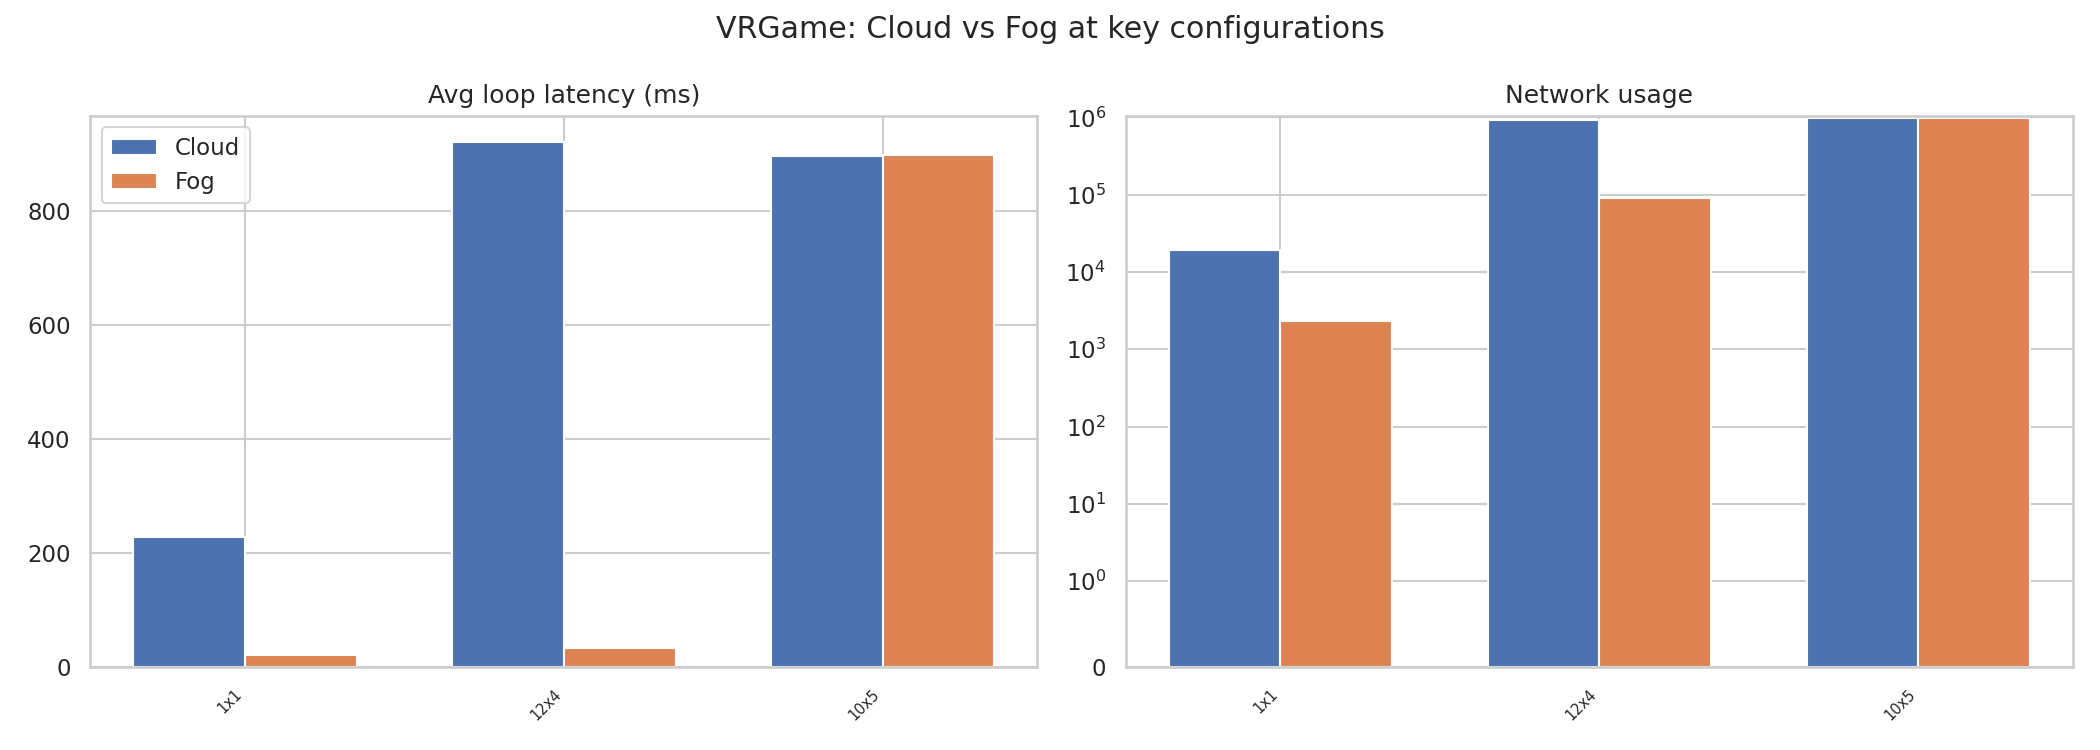
\includegraphics[width=\linewidth,keepaspectratio]{img/vrgame_key_configs.png}
    \caption{Porównanie Cloud i Fog dla trzech reprezentatywnych konfiguracji: mała skala (1$\times$1), duża skala przy niskim obciążeniu na departament (12$\times$4) oraz nasycenie routerów (10$\times$5).}
\end{figure}

Jak widać na wykresie, we wszystkich 14 konfiguracjach Fog skraca opóźnienie pętli EEG względem Cloud w 11 przypadkach. Dla najmniejszej skali 1$\times$1 latencja spada z ok. 228\,ms do ok. 20\,ms, co daje redukcję o ok. 91\%, a ruch sieciowy z ok. 19\,078 do ok. 2333 jednostek, czyli o ok. 88\% mniejszy. Przy konfiguracji 12$\times$4 redukcja opóźnienia wynosi ok. 96\%, z ok. 920\,ms do ok. 34\,ms, mimo dużej liczby departamentów --- o ile na departament przypada niewiele urządzeń mobilnych.

Przy największym obciążeniu na departament 5$\times$5, 8$\times$5, 10$\times$5, słupki Cloud i Fog zbiegają się: np. przy 10$\times$5 ok. 895\,ms vs ok. 898\,ms, co wskazuje na nasycenie zasobów routerów departamentowych. W takich konfiguracjach samo przesunięcie modułów na brzeg nie daje już przewagi interaktywnej wymaganej przez aplikację VR.

\subsection{Podsumowanie liczbowe}
\begin{table}[htbp]
\centering
\scriptsize
\setlength{\tabcolsep}{3pt}
\renewcommand{\arraystretch}{1.1}
\begin{tabularx}{\textwidth}{|>{\raggedright\arraybackslash}p{0.22\textwidth}|c|>{\raggedright\arraybackslash}p{0.20\textwidth}|>{\raggedright\arraybackslash}X|}
\hline
Scenariusz & Wiersze CSV & Główna metryka Fog & Kiedy Fog wygrywa \\
\hline
DCNS & 84 & detekcja/śledzenie, PTZ, sieć & do ok. 3 kamer/obszar \\
CrowdSensing & 56 & sieć, migracja, energia & ok. 20--50 użytkowników \\
Monitoring środowiskowy & 56 & opóźnienie, energia & we wszystkich 28 wierszach (fazy \texttt{env} i \texttt{env-sparse}) \\
VRGame & 28 & opóźnienie pętli EEG & gdy $\leq 4$ urządzenia mobilne na departament \\
\hline
\end{tabularx}
\caption{Skrótowe podsumowanie czterech scenariuszy eksperymentalnych.}
\end{table}

\section{Wnioski}
W scenariuszu DCNS najważniejsza okazała się liczba kamer przypadająca na jeden obszar, a nie łączna liczba kamer w całej infrastrukturze. Fog działa skutecznie przy ok. 3 kamerach na obszar lub mniej. Przy 5 kamerach widać już kompromis energetyczny, a przy 10 i więcej pojawia się saturacja MIPS oraz błędne odczyty opóźnień. Konfiguracja 10$\times$10 pokazuje, że przy złym wymiarowaniu Fog może w ogóle nie ukończyć pętli aplikacyjnej. Przypadki 2$\times$25 i 3$\times$10 dowodzą, że sama obecność urządzeń brzegowych nie gwarantuje korzyści.

CrowdSensing zachowuje się inaczej ze względu na mobilność. Przy małej liczbie użytkowników koszt migracji przeważa nad zyskiem z lokalnego przetwarzania. Korzyść sieciowa Fog pojawia się mniej więcej od 20 użytkowników i utrzymuje się do ok. 50, po czym między 52 a 55 użytkownikami sytuacja się odwraca. Przy dużej skali, np. 70 użytkowników, czasy migracji są zbliżone: Cloud 61{,}5\,ms, Fog 63{,}3\,ms.

Własna aplikacja monitoringu środowiskowego, ze statyczną topologią i prostszą pętlą danych, daje stabilną przewagę Fog w całym badanym zakresie. Opóźnienie spada o ok. 96--99\%, a energia o ok. 9--16\%. Faza \texttt{env-sparse} dodatkowo obniża ruch sieciowy Cloud bez pogorszenia metryk Fog. Scenariusz ten uzupełnia DCNS i CrowdSensing o przypadek IoT bez mobilności, gdzie decydujące znaczenie ma dopasowanie obciążenia do mocy bram fog.

Scenariusz VRGame pokazuje, że przy interaktywnych aplikacjach VR/EEG Fog skraca opóźnienie pętli nawet o ok. 90--96\% przy umiarkowanej skali, lecz traci przewagę przy dużej liczbie urządzeń mobilnych na departament. Wnioski te są spójne z DCNS: korzyść z brzegu zależy od tego, czy lokalne routery mają wystarczającą rezerwę MIPS.

W dalszych badaniach warto sprawdzić, czy własną aplikację można przeciążyć większą liczbą sensorów na bramę, przeanalizować koszty chmurowe przy hybrydowym placementcie oraz powtórzyć niestabilne konfiguracje DCNS przy dłuższym czasie symulacji.

\section{Wkład członków zespołu}

\subsection*{Adrian Chmiel --- część techniczna i eksperymenty}
\begin{itemize}[noitemsep,topsep=2pt]
    \item konfiguracja forka iFogSim i środowiska uruchomieniowego
    \item rozszerzenie aplikacji DCNS, CrowdSensing i VRGame o argumenty wiersza poleceń oraz eksport metryk do CSV
    \item implementacja aplikacji monitoringu środowiskowego, w tym parametru selektywności detektora anomalii
    \item modyfikacje logiki placementu Cloud i Fog dla wszystkich scenariuszy
    \item przygotowanie skryptu eksperymentalnego, uruchomienie symulacji i zebranie surowych wyników
\end{itemize}

\subsection*{Michał Bogucki --- analiza wyników}
\begin{itemize}[noitemsep,topsep=2pt]
    \item przetworzenie wyników z plików CSV i przygotowanie wykresów
    \item porównanie strategii Cloud i Fog oraz interpretacja kompromisów między opóźnieniem, ruchem sieciowym, energią i czasem migracji
    \item identyfikacja efektów zaburzających pomiar, takich jak nasycenie MIPS, nieukończone pętle, mylące odczyty opóźnień
    \item redakcja sekcji \emph{Eksperymenty}, \emph{Wyniki} oraz \emph{Wnioski}
\end{itemize}

\subsection*{Szymon Bedeniczuk --- teoria i dokumentacja}
\begin{itemize}[noitemsep,topsep=2pt]
    \item opis fog computingu oraz narzędzia iFogSim w sekcjach \emph{Wprowadzenie} oraz \emph{Cel i Zastosowanie}
    \item opis architektury warstwowej oraz interfejsu oprogramowania
    \item przegląd literatury wraz z powiązaniem publikacji z eksperymentami projektu
    \item opracowanie bibliografii oraz złożenie i finalna redakcja raportu
\end{itemize}

\clearpage
\printbibliography
\pagestyle{plain}

\clearpage
\section*{Załącznik: Spis modyfikacji kodu względem oryginalnego repozytorium iFogSim2}
\addcontentsline{toc}{section}{Załącznik: Spis modyfikacji kodu}
Poniżej zestawiono zmiany wprowadzone w naszym forku względem oryginalnego repozytorium (\url{https://github.com/Cloudslab/iFogSim}).

\subsection*{Aplikacje perfeval}
Plik \texttt{DCNSFog.java} pochodzi z oryginalnego repozytorium iFogSim (autor: Harshit Gupta). W forku dodaliśmy argumenty wiersza poleceń (\texttt{--areas}, \texttt{--cameras}, \texttt{--cloud}) oraz eksport wyników do CSV z kolumnami \texttt{Loop1Latency} (detekcja i śledzenie) i \texttt{Loop2Latency} (sterowanie PTZ).

Plik \texttt{CrowdSensing\_Microservices\_RandomMobility\_Clustering.java} również pochodzi z oryginalnego repozytorium. Rozszerzyliśmy go o parametry \texttt{--users} i \texttt{--cloud-only} oraz eksport metryk \texttt{AvgLoopLatency} i \texttt{MigrationTime} do pliku CSV.

Plik \texttt{EnvironmentalMonitoringFog.java} to nasza własna aplikacja projektu. Modeluje monitoring środowiskowy: sensor $\rightarrow$ filtr $\rightarrow$ detektor anomalii $\rightarrow$ alarm, obsługuje parametry \texttt{--gateways}, \texttt{--sensors-per-gateway}, \texttt{--cloud} i klasycznie zapisuje wyniki do pliku CSV. Dodano parametr \texttt{--anomaly-selectivity} (domyślnie 1,0) oraz kolumnę \texttt{AnomalySelectivity} w CSV, co pozwala modelować rzadkie anomalie przez \texttt{FractionalSelectivity} na wyjściu detektora anomalii.

Plik \texttt{VRGameFog.java} pochodzi z oryginalnego repozytorium (autor: Harshit Gupta). W forku rozszerzyliśmy go o argumenty \texttt{--departments}, \texttt{--mobiles-per-dept}, \texttt{--cloud} oraz eksport wyników z kolumnami \texttt{AvgLoopLatency}, \texttt{NetworkUsage}, \texttt{TotalEnergy} i \texttt{CloudExecutionCost}.

\subsection*{Logika placementu}
W forku poprawiono trzy klasy odpowiedzialne za rozmieszczanie modułów: ModulePlacementEdgewards (używana w DCNS Fog i monitoringu środowiskowego), ClusteredMicroservicePlacementLogic oraz MicroservicesMobilityClusteringController (CrowdSensing Fog).

\subsection*{Infrastruktura eksperymentalna}
Skrypt \texttt{scripts/run\_experiments.sh} uruchamia 224 warianty symulacji (84 DCNS, 56 CrowdSensing, 56 monitoring środowiskowy, 28 VRGame), kompiluje potrzebne klasy, stosuje limit czasu 10 minut na wariant, zapisuje logi w \texttt{logs/} i przenosi pliki CSV do katalogu \texttt{results/}.

Zaktualizowano również \texttt{README.md} z instrukcją budowy i uruchamiania eksperymentów w naszym forku.

\end{document}
